\documentclass{standalone}

\usepackage[english]{babel}

% to use colors

\usepackage{xcolor}

% to define font size

\usepackage{amsfonts}
\usepackage{ulem}
\usepackage{moresize}
\usepackage{anyfontsize}

% to use tikz and its libraries

\usepackage{tikz-timing}
\usepackage{tikz}

\usetikzlibrary{backgrounds}
\usetikzlibrary{decorations.pathreplacing, positioning, calc, arrows, shapes, automata, petri, patterns}

% to use tikzmark, to place and refer to marks outside the current figure

\tikzset{every picture/.style={remember picture}}

% styles for transitions

\tikzset{transition/.append style={fill=black!20, thick}}
\tikzset{transition/.append style={fill=black!20, thick}}

% styles for test and inhib arcs.

\tikzstyle{test}=[pre, *-]
\tikzstyle{inhib}=[pre, o-]

%%%%%%%%%%%%%%%%%%%%%%%%%%%%%%%%%%%%%%%%%%%%%%%%%%
%                  BEGIN DOCUMENT                %
%%%%%%%%%%%%%%%%%%%%%%%%%%%%%%%%%%%%%%%%%%%%%%%%%%

\begin{document}

\newcommand\nodesep{(1,0)}

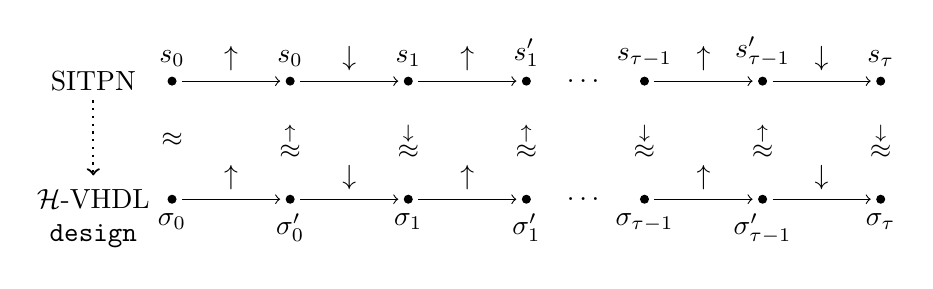
\begin{tikzpicture}

  % SITPN state nodes

  \node (sitpn) {SITPN};
  \node[draw, circle, inner sep=1pt, fill=black, label={above:$s_0$}] (s0) at ($(sitpn)+(1,0)$){};

  \node[draw, circle, inner sep=1pt, fill=black, label={above:$s_0$}] (s0bis) at ($(s0)+(1.5,0)$) {};
  \node[draw, circle, inner sep=1pt, fill=black, label={above:$s_1$}] (s1) at ($(s0bis)+(1.5,0)$) {};
  \node[draw, circle, inner sep=1pt, fill=black, label={above:$s'_1$}] (s1p) at ($(s1)+(1.5,0)$) {};
  \node[draw, circle, inner sep=1pt, fill=black, label={above:$s_{\tau-1}$}] (staumo) at ($(s1p)+(1.5,0)$) {};
  
  \node at ($(s1p.east)!.5!(staumo.west)$) {\dots};

  \node[draw, circle, inner sep=1pt,fill=black, label={above:$s'_{\tau-1}$}] (staumop) at ($(staumo)+(1.5,0)$) {};
  \node[draw, circle, inner sep=1pt, fill=black, label={above:$s_\tau$}] (stau) at ($(staumop)+(1.5,0)$) {};

  \draw ($(s0.east)+(2pt,0)$) edge[->] node [midway, above] {$\uparrow$} ($(s0bis.west)-(2pt,0)$);
  \draw ($(s0bis.east)+(2pt,0)$) edge[->] node [midway, above] {$\downarrow$} ($(s1.west)-(2pt,0)$);
  \draw ($(s1.east)+(2pt,0)$) edge[->] node [midway, above] {$\uparrow$} ($(s1p.west)-(2pt,0)$);
  \draw ($(staumo.east)+(2pt,0)$) edge[->] node [midway, above] {$\uparrow$} ($(staumop.west)-(2pt,0)$);
  \draw ($(staumop.east)+(2pt,0)$) edge[->] node [midway, above] {$\downarrow$} ($(stau.west)-(2pt,0)$);

  % VHDL design nodes

  \node (vhdld) at ($(sitpn.south)-(0,1.5)$) {
    \begin{tabular}{@{}c@{}}
      $\mathcal{H}$-VHDL \\
      $\mathtt{design}$ \\
    \end{tabular}
  };
  \draw[dotted, ->, thick] (sitpn.south) -- (vhdld.north);

  % HVHDL Design TRACE
  
  \node[draw, circle, inner sep=1pt, fill=black, label={below: $\sigma_0$}] (sig0) at ($(s0)-(0,1.5)$) {};
  \node[draw, circle, inner sep=1pt, fill=black, label={below: $\sigma'_{0}$}] (sig0prime) at ($(sig0)+(1.5,0)$) {};
  \draw ($(sig0.east)+(2pt,0)$) edge[->] node [midway, above] {$\uparrow$} ($(sig0prime.west)-(2pt,0)$);

  \node[draw, circle, inner sep=1pt, fill=black, label={below: $\sigma_1$}] (sig1) at ($(sig0prime)+(1.5,0)$) {};
  \draw ($(sig0prime.east)+(2pt,0)$) edge[->] node [midway, above] {$\downarrow$} ($(sig1.west)-(2pt,0)$);
  
  \node[draw, circle, inner sep=1pt, fill=black, label={below: $\sigma'_1$}] (sig1prime) at ($(sig1)+(1.5,0)$) {};
  \draw ($(sig1.east)+(2pt,0)$) edge[->] node [midway, above] {$\uparrow$} ($(sig1prime.west)-(2pt,0)$);

  \node[draw, circle, inner sep=1pt, fill=black, label={below: $\sigma_{\tau-1}$}] (sigtaumo) at ($(sig1prime)+(1.5,0)$) {};
  \node at ($(sig1prime)!.5!(sigtaumo)$) {\dots};

  \node[draw, circle, inner sep=1pt, fill=black, label={below: $\sigma'_{\tau-1}$}] (sigtaumoprime) at ($(sigtaumo)+(1.5,0)$) {};  
  \node[draw, circle, inner sep=1pt, fill=black, label={below: $\sigma_\tau$}] (sigtau) at ($(sigtaumoprime)+(1.5,0)$) {};

  \draw ($(sigtaumo.east)+(2pt,0)$) edge[->] node [midway, above] {$\uparrow$} ($(sigtaumoprime.west)-(2pt,0)$);
  \draw ($(sigtaumoprime.east)+(2pt,0)$) edge[->] node [midway, above] {$\downarrow$} ($(sigtau.west)-(2pt,0)$);

  % SIM. REL. SYMBOLS
  
  \node at ($(s0.south)!.5!(sig0.north)$) {$\approx$};
  \node at ($(s0bis.south)!.5!(sig0prime.north)$) {$\stackrel{\uparrow}{\approx}$};
  \node at ($(s1.south)!.5!(sig1.north)$) {$\stackrel{\downarrow}{\approx}$};
  \node at ($(s1p.south)!.5!(sig1prime.north)$) {$\stackrel{\uparrow}{\approx}$};
  \node at ($(staumo.south)!.5!(sigtaumo.north)$) {$\stackrel{\downarrow}{\approx}$};
  \node at ($(staumop.south)!.5!(sigtaumoprime.north)$) {$\stackrel{\uparrow}{\approx}$};
  \node at ($(stau.south)!.5!(sigtau.north)$) {$\stackrel{\downarrow}{\approx}$};
  
\end{tikzpicture}

\end{document}